% =====================================================================
% Anexo E: evidencia visual del preprocesamiento (Unidad 1) sobre PL13 y PL7.
% Movida desde el capitulo 4 para mantener directo el cuerpo del documento.
% =====================================================================

\section*{Anexo E. Evidencia visual del preprocesamiento}
\label{sec:anexo-evidencia-m1}
\phantomsection\addcontentsline{toc}{section}{Anexo E. Evidencia visual del preprocesamiento}

% Numeracion propia del anexo: figuras y tablas como E.n
\setcounter{figure}{0}\renewcommand{\thefigure}{E.\arabic{figure}}
\setcounter{table}{0}\renewcommand{\thetable}{E.\arabic{table}}

Este anexo recoge la evidencia visual de los pasos 1 a 5 de la Unidad~1
(Sección~\ref{sec:res-unidad1}) sobre los escaneos PL13 y PL7 de la Catedral de
Lima. Los conteos y tiempos están en la Tabla~\ref{tab:m1-metadatos}.

\FloatBarrier
\subsubsection*{Paso 1. Carga}

Cada escaneo se lee en dos bloques, en cerca de un segundo (\texttt{n\_crudo}
en la Tabla~\ref{tab:m1-metadatos}). Es la data de entrada tal como la entrega el
escáner, con su color real y sin ninguna corrección
(Figura~\ref{fig:m1-paso1}).

\begin{figure}[!htbp]
\centering
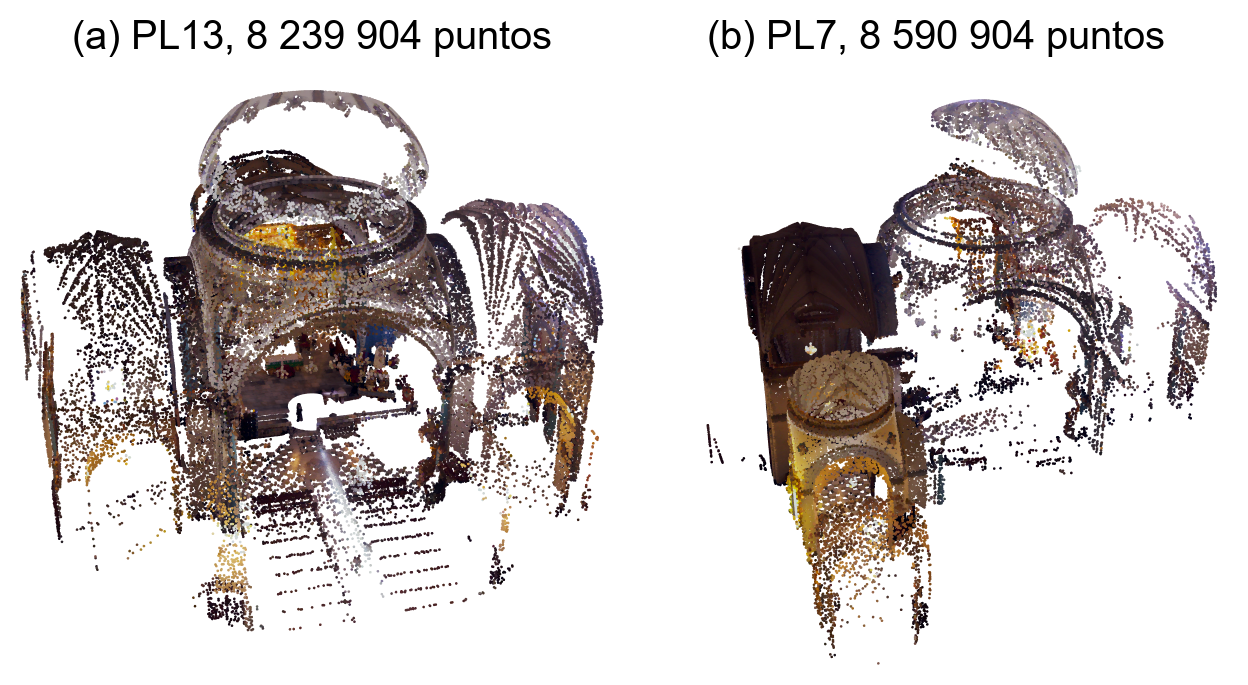
\includegraphics[width=0.75\linewidth]{imagenes/m1_paso1_carga.png}
\caption[PL13 y PL7 tras la carga]{PL13 y PL7 tras la carga. Elaboración propia con el visor del proyecto (\hyperref[sec:anexo-software]{Anexo~A}).}
\label{fig:m1-paso1}
\end{figure}

\FloatBarrier
\subsubsection*{Paso 2. Centrado}

Los dos escaneos son vecinos, sus centros están a unos 17\,m uno de otro, pero
cada uno se centra en su propio origen (Tabla~\ref{tab:m1-centrado}). Este paso no lleva imagen
porque la nube se ve igual antes y después, solo cambian los números de los
ejes.

\begin{table}[!htbp]
\centering
\setstretch{1}\small
\caption[Coordenadas de PL13 y PL7 antes y después del centrado]{Coordenadas de PL13 y PL7 antes y después del centrado, en metros. Elaboración propia.}
\label{tab:m1-centrado}
\begin{tabularx}{\linewidth}{@{}ll>{\raggedright\arraybackslash\hsize=1.00\hsize}Xll@{}}
\toprule
\textbf{Escaneo} & \textbf{Eje} & \textbf{Antes, en UTM} & \textbf{Centro} & \textbf{Después} \\
\midrule
PL13 & $x$ & 278\,772{,}08 a 278\,804{,}90 & 278\,788{,}49 & $-16{,}41$ a $16{,}41$ \\
     & $y$ & 8\,667\,747{,}60 a 8\,667\,779{,}68 & 8\,667\,763{,}64 & $-16{,}04$ a $16{,}04$ \\
     & $z$ & 161{,}61 a 183{,}89 & 172{,}75 & $-11{,}14$ a $11{,}14$ \\
\midrule
PL7  & $x$ & 278\,775{,}30 a 278\,826{,}64 & 278\,800{,}97 & $-25{,}67$ a $25{,}67$ \\
     & $y$ & 8\,667\,724{,}83 a 8\,667\,780{,}02 & 8\,667\,752{,}42 & $-27{,}60$ a $27{,}60$ \\
     & $z$ & 159{,}36 a 188{,}83 & 174{,}10 & $-14{,}73$ a $14{,}73$ \\
\bottomrule
\end{tabularx}
\end{table}

\FloatBarrier
\subsubsection*{Paso 3. Filtrado SOR}

En PL13 se descartan 219\,108 puntos, el 2{,}66\,\%, y en PL7 406\,485, el
4{,}73\,\% (\texttt{n\_sor} en la Tabla~\ref{tab:m1-metadatos}). El filtrado tardó
cerca de nueve segundos en PL13 y doce en PL7.

En ambos escaneos los descartes se concentran en las zonas ralas, lejos del
escáner (Figura~\ref{fig:m1-paso3}). PL7
descarta casi el doble que PL13, y en la figura se ve que también tiene más
zonas ralas.

\begin{figure}[!htbp]
\centering
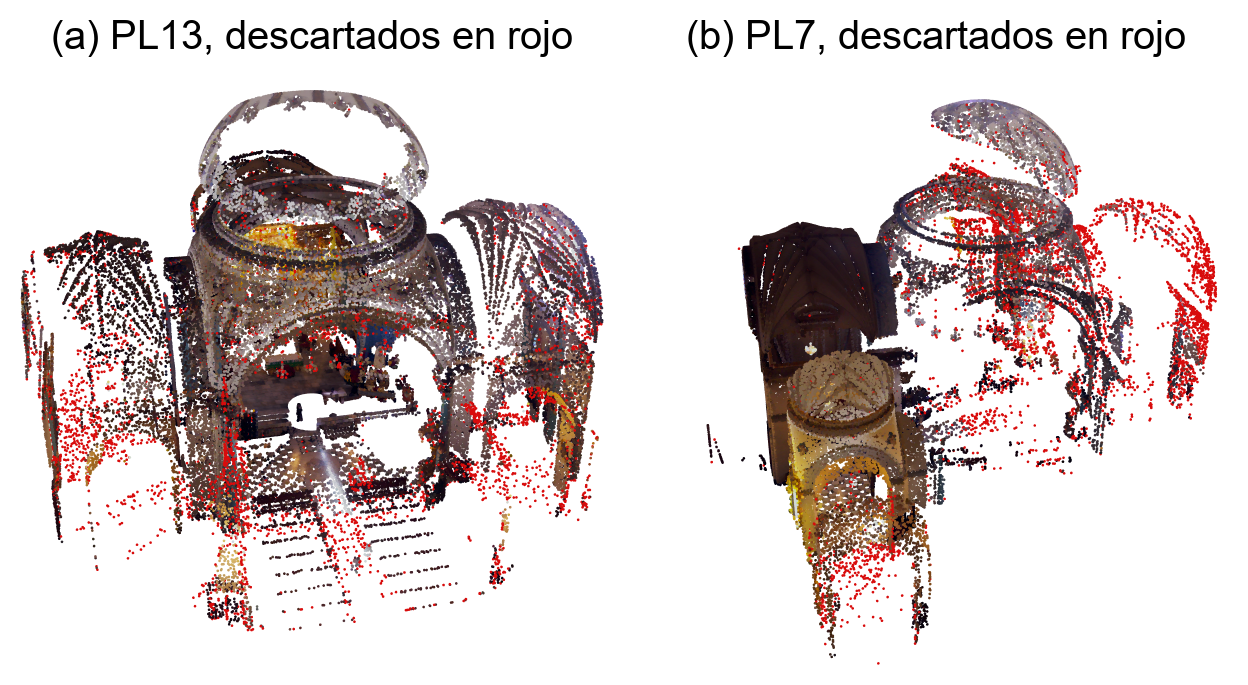
\includegraphics[width=0.85\linewidth]{imagenes/m1_paso3_sor.png}
\caption[PL13 y PL7 con los puntos descartados por el SOR en rojo]{PL13 y PL7 con los puntos descartados por el SOR en rojo. Elaboración propia con el visor del proyecto (\hyperref[sec:anexo-software]{Anexo~A}).}
\label{fig:m1-paso3}
\end{figure}

\FloatBarrier
\subsubsection*{Paso 4. Voxelización}

En PL13 quedan como representantes el 10{,}01\,\% de los puntos que salieron
del filtrado, y en PL7 el 7{,}46\,\% (\texttt{n\_voxel} en la
Tabla~\ref{tab:m1-metadatos})
(Figuras~\ref{fig:m1-paso4-pl13} y~\ref{fig:m1-paso4}). De cerca
(Figuras~\ref{fig:cubo-pl13} y~\ref{fig:cubo-pl7}), en el cubo de PL13 los
37\,777 puntos de la entrada quedan en 1\,159 representantes, y en el de PL7 los
48\,098 quedan en 921. En el cubo de PL7 la entrada contiene varias superficies
paralelas separadas por pocos centímetros, que en la salida ya no se distinguen,
como anticipa el \enlace{sec:u1-p4}{Paso~4}. En los cubos se dibujan todos los puntos, con el color aclarado por un
factor de 2{,}2. Los dos cubos se eligieron con el mismo criterio, tener muchos
puntos y superficies en varias orientaciones. El de PL13 va de $x=-3$ a $-2$\,m,
de $y=7$ a $8$\,m y de $z=-8$ a $-7$\,m, y el de PL7 de $x=-19$ a $-18$\,m, de
$y=-3$ a $-2$\,m y de $z=-12$ a $-11$\,m, en las coordenadas centradas de cada
escaneo.

\begin{figure}[!htbp]
\centering
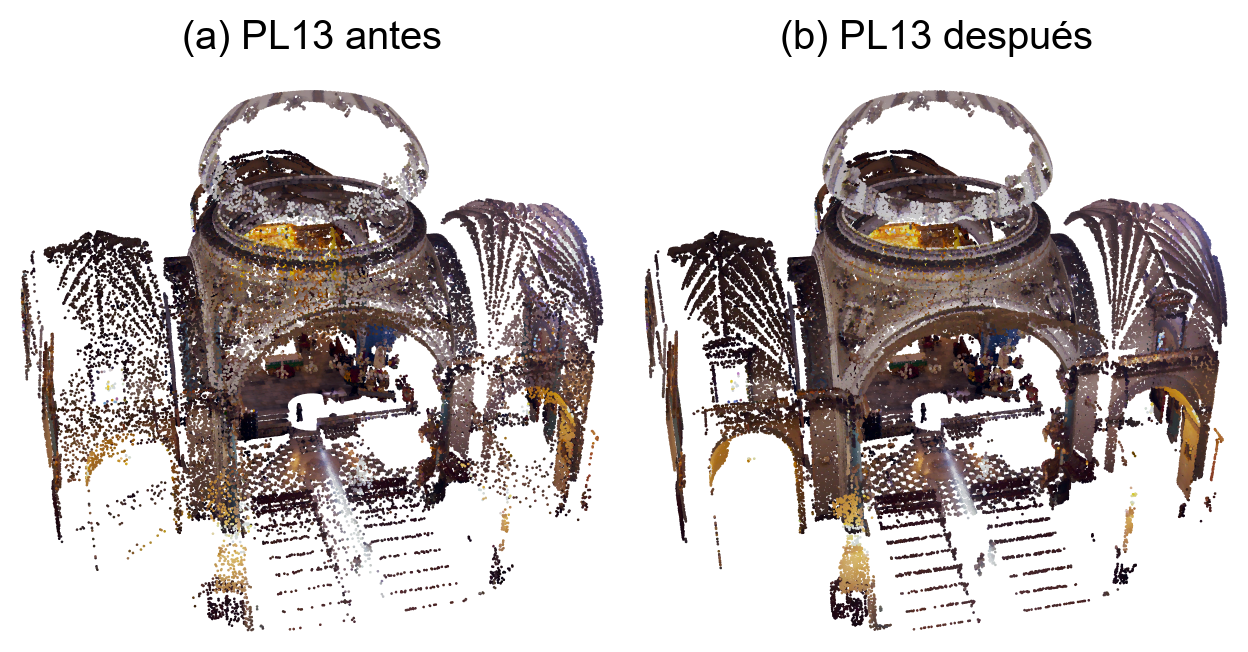
\includegraphics[width=0.75\linewidth]{imagenes/m1_paso4_voxel_completo_pl13.png}
\caption[PL13 antes y después de la voxelización]{PL13 antes y después de la voxelización. Elaboración propia con el visor del proyecto (\hyperref[sec:anexo-software]{Anexo~A}).}
\label{fig:m1-paso4-pl13}
\end{figure}

\begin{figure}[!htbp]
\centering
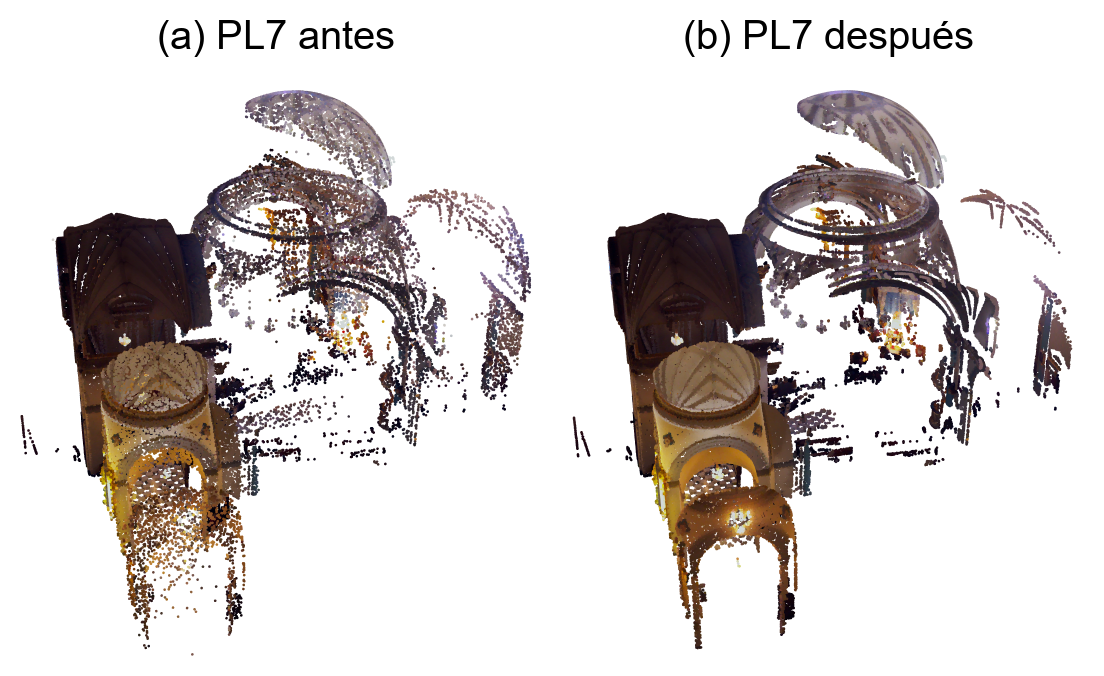
\includegraphics[width=0.75\linewidth]{imagenes/m1_paso4_voxel_completo.png}
\caption[PL7 antes y después de la voxelización]{PL7 antes y después de la voxelización. Elaboración propia con el visor del proyecto (\hyperref[sec:anexo-software]{Anexo~A}).}
\label{fig:m1-paso4}
\end{figure}

\begin{figure}[!htbp]
\centering
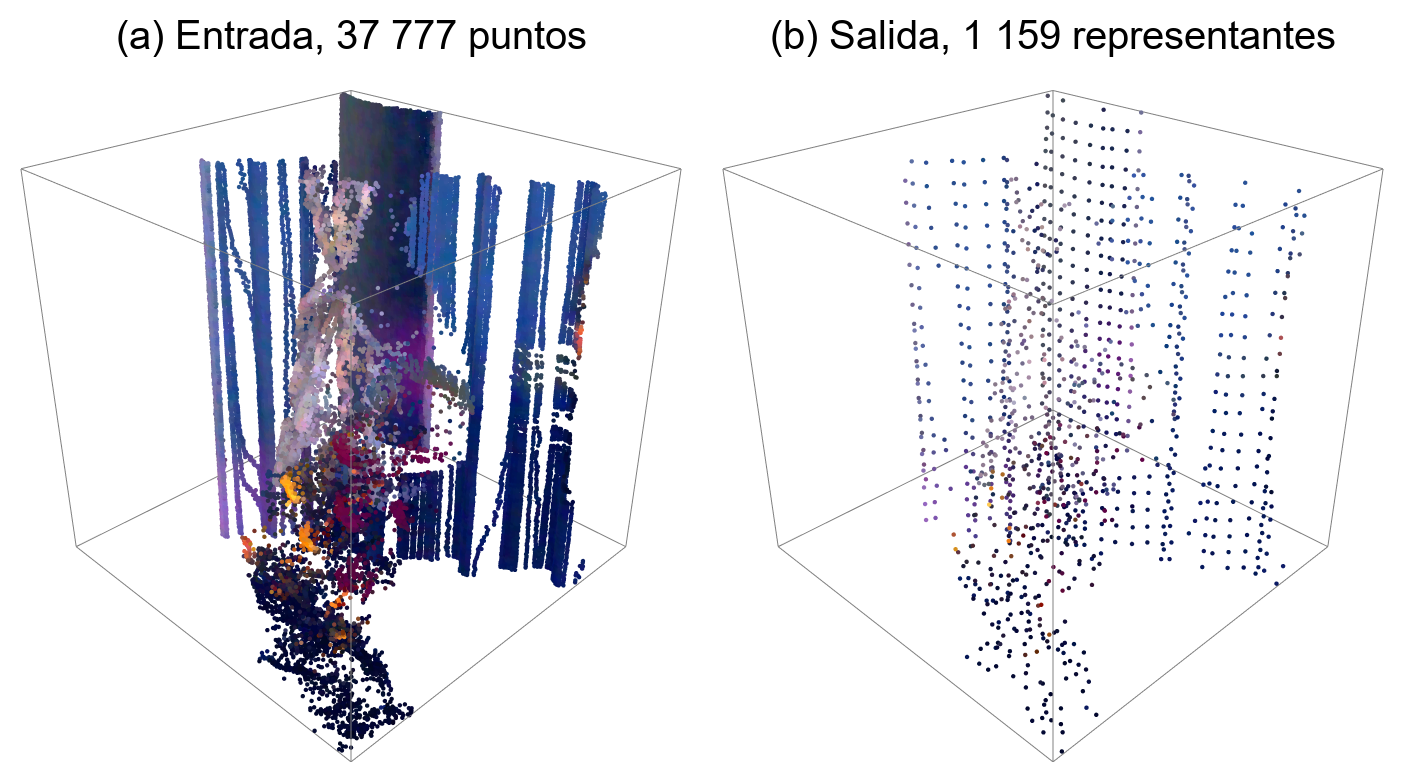
\includegraphics[width=0.6\linewidth]{imagenes/m1_paso4_voxel_cubo_pl13.png}
\caption[Cubo de 1\,m de PL13 antes y después de la voxelización]{Cubo de 1\,m de PL13 antes y después de la voxelización. Elaboración propia con el visor del proyecto (\hyperref[sec:anexo-software]{Anexo~A}).}
\label{fig:cubo-pl13}
\end{figure}

\begin{figure}[!htbp]
\centering
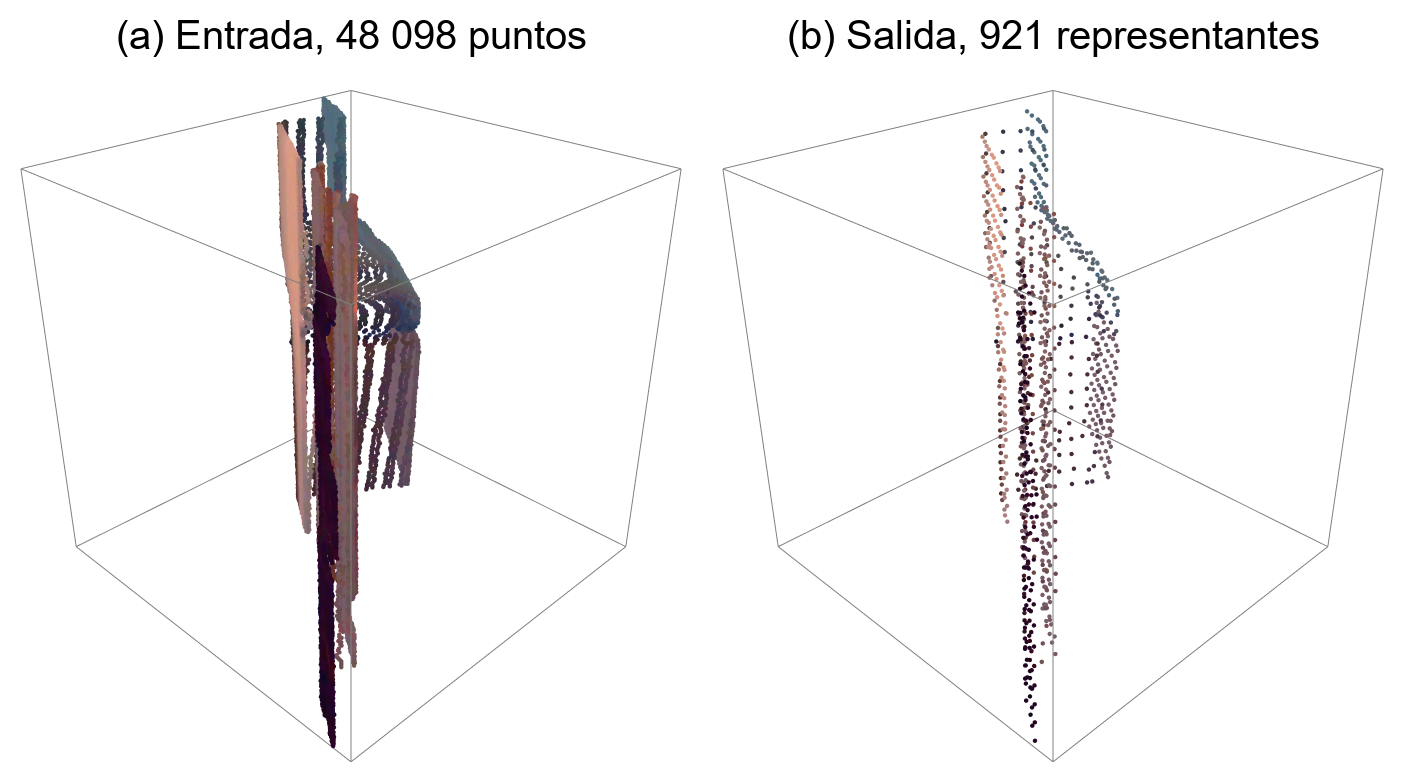
\includegraphics[width=0.6\linewidth]{imagenes/m1_paso4_voxel_cubo.png}
\caption[Cubo de 1\,m de PL7 antes y después de la voxelización]{Cubo de 1\,m de PL7 antes y después de la voxelización. Elaboración propia con el visor del proyecto (\hyperref[sec:anexo-software]{Anexo~A}).}
\label{fig:cubo-pl7}
\end{figure}

\FloatBarrier
\subsubsection*{Paso 5. Normales}

Las superficies con la misma orientación toman el mismo tono
(Figura~\ref{fig:m1-paso5}). En las bóvedas el
color cambia de forma gradual, siguiendo su curvatura. En las zonas ralas, lejos
del escáner, aparecen manchas de colores mezclados. Es la misma zona en la que el
filtrado del Paso~3 concentró sus descartes.

\begin{figure}[!htbp]
\centering
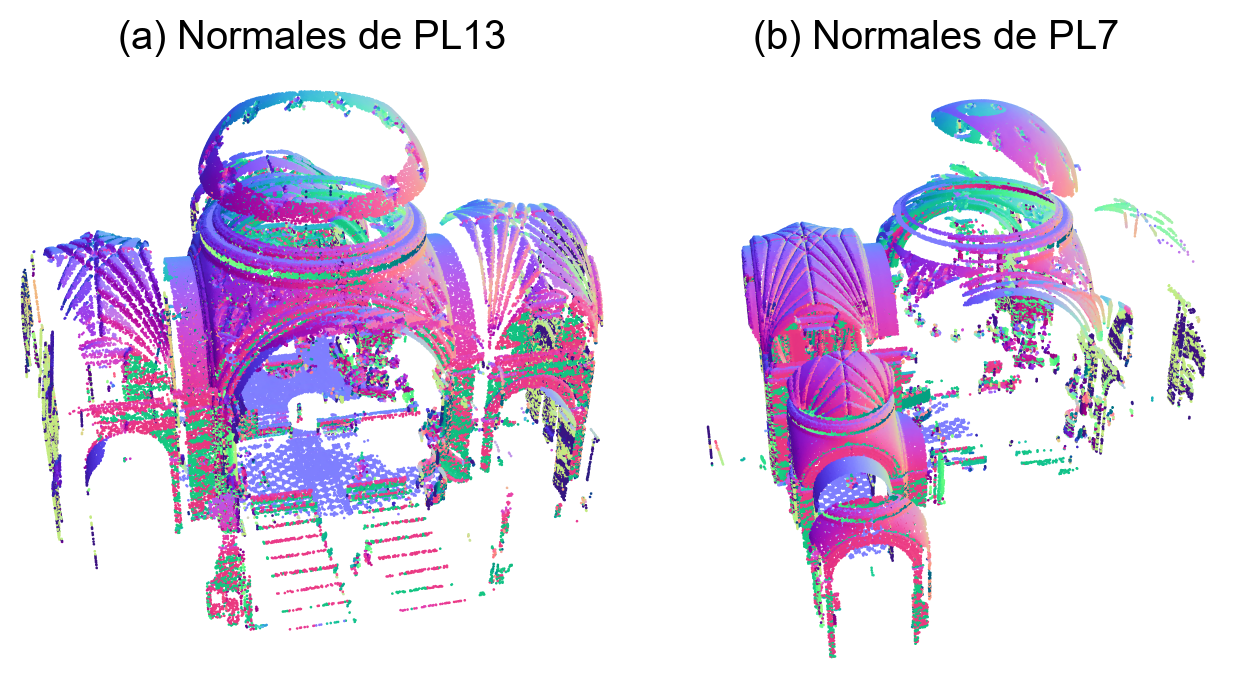
\includegraphics[width=0.75\linewidth]{imagenes/m1_paso5_normales.png}
\caption[Normales de PL13 y PL7 como color]{Normales de PL13 y PL7 como color. Elaboración propia con el visor del proyecto (\hyperref[sec:anexo-software]{Anexo~A}).}
\label{fig:m1-paso5}
\end{figure}

